% -*- root: article.tex -*-
Durante o processo de codificação emergiram 23 boas e más práticas. Classificamos essas práticas de acordo com sua recorrência: alta (acima de 20 respostas), média (de 8 a 20 respostas) e baixa (de 3 a 7 respostas). Obtivemos 4 de alta recorrência, 14 de média e 5 de baixa. Por limitações de espaço, neste artigo só apresentamos as de alta e média recorrência porém o catálogo completo pode ser consultado em nosso apêndice online.

% ou baixíssima (menos de 3 respostas). 
% Na Figura \ref{fig:CategoriaXRecorrencia} é possível observar a distribuição das práticas de acordo com sua recorrência. 

% \begin{figure}[!htb]
% 	\centering
% 	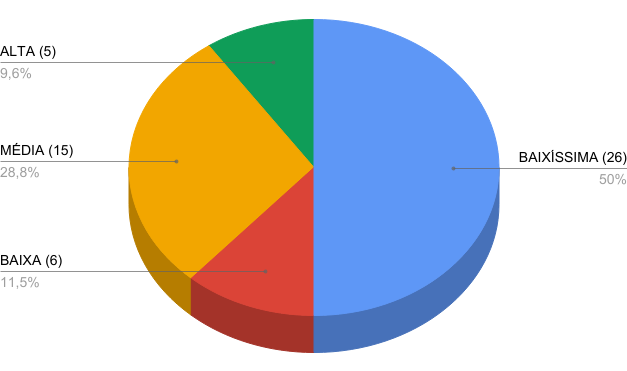
\includegraphics[width=0.45\textwidth]{grafico-recorrencia.png}
% 	\caption{Distribuição das práticas vs. recorrência}
% 	\label{fig:CategoriaXRecorrencia}
% \end{figure}

A Tabela \ref{tab:Categories} apresenta o total de ocorrências de cada prática (\textit{S1}). A última linha da tabela, \textbf{\#Categorias}, apresenta quantas categorias emergiram de cada questão, como cada questão está diretamente ligada a um elemento do \textit{front-end} Android, podemos interpretá-la da seguinte forma: \emph{quais são os pontos de atenção a serem analisados em determinado elemento Android?} A última coluna da tabela, \textbf{\#Q}, apresenta em quantas questões cada categoria surgiu, podemos interpretá-la da seguinte forma: \emph{com base na categoria, quais elementos devem ser investigados?}. 

% O cheiro de código \emph{Classe Deus/Longa} \cite{Riel, RefactoringFowler1999} são conceitos pré-existentes e portanto não são tratados neste artigo. 

% e Herança \cite{WikipediaInhiritance}
% Quando se criam categorizações para auxiliar desenvolvedores a identificar pontos de atenção a serem avaliados e onde este pontos devem ser investigados especificamente no código, pensando em qualidade de código dá-se o nome de \textit{smells}. Portanto, nesta seção iremos compilar este conjunto de Android \textit{code smells} que identificamos através das categorizações.


\begin{table*}
\centering
\footnotesize
\begin{tabular}{@{}p{4.2cm}p{0.3cm}p{.2cm}p{.2cm}p{.2cm}p{.2cm}p{.2cm}p{.2cm}p{.2cm}p{.2cm}p{.2cm}p{.4cm}p{.4cm}p{.4cm}p{.4cm}p{.4cm}p{.4cm}p{.4cm}p{.4cm}p{.4cm}p{0.2cm}@{}}
\toprule
\textbf{Recorrência/Prática} & \multicolumn{1}{c}{\textbf{\#T}} & Q1 & Q2 & Q3 & Q4 & Q5 & Q6 & Q7 & Q8 & Q9 & Q10 & Q11 & Q12 & Q13 & Q14 & Q15 & Q16 & Q17 & Q18 &  \multicolumn{1}{c}{\textbf{\#R}} \\
\hline
\multicolumn{2}{l}{\scriptsize{\textbf{ALTA RECORRÊNCIA (4)}}} \\
\textsc{Lógica Em Classes de UI}					& \multicolumn{1}{c}{60} 	& \multicolumn{1}{c}{14} 	& \multicolumn{1}{c}{15} 	& \multicolumn{1}{c}{8}		& \multicolumn{1}{c}{8}		& \multicolumn{1}{c}{6}		& \multicolumn{1}{c}{8}		& \multicolumn{1}{c}{--}	& \multicolumn{1}{c}{1}		& \multicolumn{1}{c}{--}	& \multicolumn{1}{c}{--}	& \multicolumn{1}{c}{--}	& \multicolumn{1}{c}{--}	& \multicolumn{1}{c}{--}	& \multicolumn{1}{c}{--}	& \multicolumn{1}{c}{--}	& \multicolumn{1}{c}{--}	& \multicolumn{1}{c}{--} 	& \multicolumn{1}{c}{--}	& \multicolumn{1}{c}{7} \\
\textsc{Nome de Recurso Despadronizado}		& \multicolumn{1}{c}{24} 	& \multicolumn{1}{c}{1} 	& \multicolumn{1}{c}{--} 	& \multicolumn{1}{c}{--}	& \multicolumn{1}{c}{--}	& \multicolumn{1}{c}{--}	& \multicolumn{1}{c}{--}	& \multicolumn{1}{c}{--}	& \multicolumn{1}{c}{--}	& \multicolumn{1}{c}{3}		& \multicolumn{1}{c}{2}		& \multicolumn{1}{c}{3}		& \multicolumn{1}{c}{2}		& \multicolumn{1}{c}{8}		& \multicolumn{1}{c}{2}		& \multicolumn{1}{c}{3}		& \multicolumn{1}{c}{--}	& \multicolumn{1}{c}{--} 	& \multicolumn{1}{c}{--}	& \multicolumn{1}{c}{8} \\
\textsc{Recurso Mágico}										& \multicolumn{1}{c}{23} 	& \multicolumn{1}{c}{--} 	& \multicolumn{1}{c}{--} 	& \multicolumn{1}{c}{--}	& \multicolumn{1}{c}{--}	& \multicolumn{1}{c}{--}	& \multicolumn{1}{c}{--}	& \multicolumn{1}{c}{--}	& \multicolumn{1}{c}{--}	& \multicolumn{1}{c}{4}		& \multicolumn{1}{c}{2}		& \multicolumn{1}{c}{1}		& \multicolumn{1}{c}{1}		& \multicolumn{1}{c}{9}		& \multicolumn{1}{c}{6}		& \multicolumn{1}{c}{--}	& \multicolumn{1}{c}{--}	& \multicolumn{1}{c}{--} 	& \multicolumn{1}{c}{--}	& \multicolumn{1}{c}{6} \\
\textsc{Layout Profundamente Aninhado}		& \multicolumn{1}{c}{21} 	& \multicolumn{1}{c}{--} 	& \multicolumn{1}{c}{--} 	& \multicolumn{1}{c}{--}	& \multicolumn{1}{c}{--}	& \multicolumn{1}{c}{1}		& \multicolumn{1}{c}{--}	& \multicolumn{1}{c}{--}	& \multicolumn{1}{c}{--}	& \multicolumn{1}{c}{9}		& \multicolumn{1}{c}{9}		& \multicolumn{1}{c}{--}	& \multicolumn{1}{c}{--}	& \multicolumn{1}{c}{--}	& \multicolumn{1}{c}{--}	& \multicolumn{1}{c}{--}	& \multicolumn{1}{c}{--}	& \multicolumn{1}{c}{1} 	& \multicolumn{1}{c}{1}		& \multicolumn{1}{c}{5} \\

\vspace{1sp} \\
\multicolumn{2}{l}{\scriptsize{\textbf{MÉDIA RECORRÊNCIA (14)}}} \\ 
\textsc{Classes de UI Acopladas}           	& \multicolumn{1}{c}{18} 	& \multicolumn{1}{c}{--} 	& \multicolumn{1}{c}{2} 	& \multicolumn{1}{c}{4}	 	& \multicolumn{1}{c}{6} 	& \multicolumn{1}{c}{--} 	& \multicolumn{1}{c}{3} 	& \multicolumn{1}{c}{1} 	& \multicolumn{1}{c}{2} 	& \multicolumn{1}{c}{--} 	& \multicolumn{1}{c}{--} 	& \multicolumn{1}{c}{--} 	& \multicolumn{1}{c}{--} 	& \multicolumn{1}{c}{--} 	& \multicolumn{1}{c}{--} 	& \multicolumn{1}{c}{--}	& \multicolumn{1}{c}{--} 	& \multicolumn{1}{c}{--} 	& \multicolumn{1}{c}{--} 	& \multicolumn{1}{c}{6} \\
\textsc{Comportamento Suspeito}            	& \multicolumn{1}{c}{18} 	& \multicolumn{1}{c}{2} 	& \multicolumn{1}{c}{2} 	& \multicolumn{1}{c}{--} 	& \multicolumn{1}{c}{--} 	& \multicolumn{1}{c}{1} 	& \multicolumn{1}{c}{2} 	& \multicolumn{1}{c}{7} 	& \multicolumn{1}{c}{3} 	& \multicolumn{1}{c}{--} 	& \multicolumn{1}{c}{--} 	& \multicolumn{1}{c}{--} 	& \multicolumn{1}{c}{--} 	& \multicolumn{1}{c}{--} 	& \multicolumn{1}{c}{--} 	& \multicolumn{1}{c}{--}	& \multicolumn{1}{c}{--} 	& \multicolumn{1}{c}{1} 	& \multicolumn{1}{c}{--} 	& \multicolumn{1}{c}{4} \\
\textsc{Mau Uso do Ciclo de Vida}          	& \multicolumn{1}{c}{15} 	& \multicolumn{1}{c}{4} 	& \multicolumn{1}{c}{3} 	& \multicolumn{1}{c}{3}	 	& \multicolumn{1}{c}{5} 	& \multicolumn{1}{c}{--} 	& \multicolumn{1}{c}{--} 	& \multicolumn{1}{c}{--} 	& \multicolumn{1}{c}{--} 	& \multicolumn{1}{c}{--} 	& \multicolumn{1}{c}{--} 	& \multicolumn{1}{c}{--} 	& \multicolumn{1}{c}{--} 	& \multicolumn{1}{c}{--} 	& \multicolumn{1}{c}{--} 	& \multicolumn{1}{c}{--}	& \multicolumn{1}{c}{--} 	& \multicolumn{1}{c}{--} 	& \multicolumn{1}{c}{--} 	& \multicolumn{1}{c}{5} \\
\textsc{Layout Longo ou Repetido}          	& \multicolumn{1}{c}{15} 	& \multicolumn{1}{c}{--} 	& \multicolumn{1}{c}{--} 	& \multicolumn{1}{c}{--} 	& \multicolumn{1}{c}{--} 	& \multicolumn{1}{c}{--} 	& \multicolumn{1}{c}{--} 	& \multicolumn{1}{c}{--} 	& \multicolumn{1}{c}{--} 	& \multicolumn{1}{c}{12} 	& \multicolumn{1}{c}{2} 	& \multicolumn{1}{c}{--} 	& \multicolumn{1}{c}{--} 	& \multicolumn{1}{c}{--} 	& \multicolumn{1}{c}{--} 	& \multicolumn{1}{c}{--}	& \multicolumn{1}{c}{--} 	& \multicolumn{1}{c}{1} 	& \multicolumn{1}{c}{--} 	& \multicolumn{1}{c}{3} \\
\textsc{Não Uso de Padrão View Holder}     	& \multicolumn{1}{c}{13} 	& \multicolumn{1}{c}{--} 	& \multicolumn{1}{c}{--} 	& \multicolumn{1}{c}{--} 	& \multicolumn{1}{c}{--} 	& \multicolumn{1}{c}{11} 	& \multicolumn{1}{c}{2} 	& \multicolumn{1}{c}{--} 	& \multicolumn{1}{c}{--} 	& \multicolumn{1}{c}{--} 	& \multicolumn{1}{c}{--} 	& \multicolumn{1}{c}{--} 	& \multicolumn{1}{c}{--} 	& \multicolumn{1}{c}{--} 	& \multicolumn{1}{c}{--} 	& \multicolumn{1}{c}{--}	& \multicolumn{1}{c}{--} 	& \multicolumn{1}{c}{--} 	& \multicolumn{1}{c}{--} 	& \multicolumn{1}{c}{2} \\
% \textsc{Classe Deus/Longa*}                	& \multicolumn{1}{c}{13} 	& \multicolumn{1}{c}{2} 	& \multicolumn{1}{c}{4} 	& \multicolumn{1}{c}{2}	 	& \multicolumn{1}{c}{2} 	& \multicolumn{1}{c}{--} 	& \multicolumn{1}{c}{1} 	& \multicolumn{1}{c}{--} 	& \multicolumn{1}{c}{1} 	& \multicolumn{1}{c}{--} 	& \multicolumn{1}{c}{--} 	& \multicolumn{1}{c}{--} 	& \multicolumn{1}{c}{1} 	& \multicolumn{1}{c}{--} 	& \multicolumn{1}{c}{--} 	& \multicolumn{1}{c}{--}	& \multicolumn{1}{c}{--} 	& \multicolumn{1}{c}{--} 	& \multicolumn{1}{c}{--} 	& \multicolumn{1}{c}{6} \\
\textsc{Não Uso de Arquiteturas Conhecidas}	& \multicolumn{1}{c}{13} 	& \multicolumn{1}{c}{4} 	& \multicolumn{1}{c}{--} 	& \multicolumn{1}{c}{2}	 	& \multicolumn{1}{c}{--} 	& \multicolumn{1}{c}{--} 	& \multicolumn{1}{c}{--} 	& \multicolumn{1}{c}{--} 	& \multicolumn{1}{c}{--} 	& \multicolumn{1}{c}{--} 	& \multicolumn{1}{c}{--} 	& \multicolumn{1}{c}{--} 	& \multicolumn{1}{c}{--} 	& \multicolumn{1}{c}{--} 	& \multicolumn{1}{c}{--} 	& \multicolumn{1}{c}{--}	& \multicolumn{1}{c}{--} 	& \multicolumn{1}{c}{6} 	& \multicolumn{1}{c}{1} 	& \multicolumn{1}{c}{4} \\
\textsc{Tamanho Único de Imagem}           	& \multicolumn{1}{c}{12} 	& \multicolumn{1}{c}{--} 	& \multicolumn{1}{c}{--} 	& \multicolumn{1}{c}{--} 	& \multicolumn{1}{c}{--} 	& \multicolumn{1}{c}{--} 	& \multicolumn{1}{c}{--} 	& \multicolumn{1}{c}{--} 	& \multicolumn{1}{c}{--} 	& \multicolumn{1}{c}{1} 	& \multicolumn{1}{c}{1} 	& \multicolumn{1}{c}{--} 	& \multicolumn{1}{c}{--} 	& \multicolumn{1}{c}{--} 	& \multicolumn{1}{c}{--} 	& \multicolumn{1}{c}{4}		& \multicolumn{1}{c}{6} 	& \multicolumn{1}{c}{--} 	& \multicolumn{1}{c}{--} 	& \multicolumn{1}{c}{7} \\
\textsc{Uso Excessivo de Fragment}         	& \multicolumn{1}{c}{11} 	& \multicolumn{1}{c}{--} 	& \multicolumn{1}{c}{--} 	& \multicolumn{1}{c}{8}	 	& \multicolumn{1}{c}{3} 	& \multicolumn{1}{c}{--} 	& \multicolumn{1}{c}{--} 	& \multicolumn{1}{c}{--} 	& \multicolumn{1}{c}{--} 	& \multicolumn{1}{c}{--} 	& \multicolumn{1}{c}{--} 	& \multicolumn{1}{c}{--} 	& \multicolumn{1}{c}{--} 	& \multicolumn{1}{c}{--} 	& \multicolumn{1}{c}{--} 	& \multicolumn{1}{c}{--}	& \multicolumn{1}{c}{--} 	& \multicolumn{1}{c}{--} 	& \multicolumn{1}{c}{--} 	& \multicolumn{1}{c}{4} \\
\textsc{Não Uso de Imagens Vetoriais}      	& \multicolumn{1}{c}{10} 	& \multicolumn{1}{c}{--} 	& \multicolumn{1}{c}{--} 	& \multicolumn{1}{c}{--} 	& \multicolumn{1}{c}{--} 	& \multicolumn{1}{c}{--} 	& \multicolumn{1}{c}{--} 	& \multicolumn{1}{c}{--} 	& \multicolumn{1}{c}{--} 	& \multicolumn{1}{c}{--} 	& \multicolumn{1}{c}{--} 	& \multicolumn{1}{c}{--} 	& \multicolumn{1}{c}{--} 	& \multicolumn{1}{c}{--} 	& \multicolumn{1}{c}{--} 	& \multicolumn{1}{c}{10}	& \multicolumn{1}{c}{--} 	& \multicolumn{1}{c}{--} 	& \multicolumn{1}{c}{--} 	& \multicolumn{1}{c}{1} \\
\textsc{Não Uso de Fragment}               	& \multicolumn{1}{c}{9} 	& \multicolumn{1}{c}{3} 	& \multicolumn{1}{c}{2} 	& \multicolumn{1}{c}{4}	 	& \multicolumn{1}{c}{--} 	& \multicolumn{1}{c}{--} 	& \multicolumn{1}{c}{--} 	& \multicolumn{1}{c}{--} 	& \multicolumn{1}{c}{--} 	& \multicolumn{1}{c}{--} 	& \multicolumn{1}{c}{--} 	& \multicolumn{1}{c}{--} 	& \multicolumn{1}{c}{--} 	& \multicolumn{1}{c}{--} 	& \multicolumn{1}{c}{--} 	& \multicolumn{1}{c}{--}	& \multicolumn{1}{c}{--} 	& \multicolumn{1}{c}{--} 	& \multicolumn{1}{c}{--} 	& \multicolumn{1}{c}{2} \\
\textsc{Classes de UI Fazendo IO}          	& \multicolumn{1}{c}{9} 	& \multicolumn{1}{c}{1} 	& \multicolumn{1}{c}{4} 	& \multicolumn{1}{c}{1}	 	& \multicolumn{1}{c}{2} 	& \multicolumn{1}{c}{--} 	& \multicolumn{1}{c}{1} 	& \multicolumn{1}{c}{--} 	& \multicolumn{1}{c}{--} 	& \multicolumn{1}{c}{--} 	& \multicolumn{1}{c}{--} 	& \multicolumn{1}{c}{--} 	& \multicolumn{1}{c}{--} 	& \multicolumn{1}{c}{--} 	& \multicolumn{1}{c}{--} 	& \multicolumn{1}{c}{--}	& \multicolumn{1}{c}{--} 	& \multicolumn{1}{c}{--} 	& \multicolumn{1}{c}{--} 	& \multicolumn{1}{c}{4} \\
\textsc{Longo Recurso de Estilo}           	& \multicolumn{1}{c}{8} 	& \multicolumn{1}{c}{--} 	& \multicolumn{1}{c}{--} 	& \multicolumn{1}{c}{--} 	& \multicolumn{1}{c}{--} 	& \multicolumn{1}{c}{--} 	& \multicolumn{1}{c}{--} 	& \multicolumn{1}{c}{--} 	& \multicolumn{1}{c}{--} 	& \multicolumn{1}{c}{--} 	& \multicolumn{1}{c}{--} 	& \multicolumn{1}{c}{5} 	& \multicolumn{1}{c}{3} 	& \multicolumn{1}{c}{--} 	& \multicolumn{1}{c}{--} 	& \multicolumn{1}{c}{--}	& \multicolumn{1}{c}{--} 	& \multicolumn{1}{c}{--} 	& \multicolumn{1}{c}{--} 	& \multicolumn{1}{c}{2} \\
\textsc{Recurso de String Bagunçado}       	& \multicolumn{1}{c}{8} 	& \multicolumn{1}{c}{--} 	& \multicolumn{1}{c}{--} 	& \multicolumn{1}{c}{--} 	& \multicolumn{1}{c}{--} 	& \multicolumn{1}{c}{--} 	& \multicolumn{1}{c}{--} 	& \multicolumn{1}{c}{--} 	& \multicolumn{1}{c}{--} 	& \multicolumn{1}{c}{--} 	& \multicolumn{1}{c}{--} 	& \multicolumn{1}{c}{--} 	& \multicolumn{1}{c}{--} 	& \multicolumn{1}{c}{4} 	& \multicolumn{1}{c}{4} 	& \multicolumn{1}{c}{--}	& \multicolumn{1}{c}{--} 	& \multicolumn{1}{c}{--} 	& \multicolumn{1}{c}{--} 	& \multicolumn{1}{c}{2} \\
\textsc{Atributos de Estilo Repetidos}     	& \multicolumn{1}{c}{8} 	& \multicolumn{1}{c}{--} 	& \multicolumn{1}{c}{--} 	& \multicolumn{1}{c}{--} 	& \multicolumn{1}{c}{--} 	& \multicolumn{1}{c}{--} 	& \multicolumn{1}{c}{--} 	& \multicolumn{1}{c}{--} 	& \multicolumn{1}{c}{--} 	& \multicolumn{1}{c}{1} 	& \multicolumn{1}{c}{2} 	& \multicolumn{1}{c}{2} 	& \multicolumn{1}{c}{2} 	& \multicolumn{1}{c}{--} 	& \multicolumn{1}{c}{--} 	& \multicolumn{1}{c}{--}	& \multicolumn{1}{c}{--} 	& \multicolumn{1}{c}{1} 	& \multicolumn{1}{c}{--} 	& \multicolumn{1}{c}{5} \\

% \vspace*{1sp} \\
% \multicolumn{2}{l}{\scriptsize{\textbf{BAIXA RECORRÊNCIA (6)}}} \\
% \textsc{Activity Inexistente}								& \multicolumn{1}{c}{7}  	& \multicolumn{1}{c}{2}  	& \multicolumn{1}{c}{4}  	& \multicolumn{1}{c}{--} 	& \multicolumn{1}{c}{--} 	& \multicolumn{1}{c}{--} 	& \multicolumn{1}{c}{--} 	& \multicolumn{1}{c}{--} 	& \multicolumn{1}{c}{1} 	& \multicolumn{1}{c}{--} 	& \multicolumn{1}{c}{--} 	& \multicolumn{1}{c}{--} 	& \multicolumn{1}{c}{--} 	& \multicolumn{1}{c}{--} 	& \multicolumn{1}{c}{--} 	& \multicolumn{1}{c}{--} 	& \multicolumn{1}{c}{--} 	& \multicolumn{1}{c}{--} 	& \multicolumn{1}{c}{--} 	& \multicolumn{1}{c}{3} \\
% \textsc{Imagem Dispensável}									& \multicolumn{1}{c}{6}  	& \multicolumn{1}{c}{--}  	& \multicolumn{1}{c}{--}  	& \multicolumn{1}{c}{--} 	& \multicolumn{1}{c}{--} 	& \multicolumn{1}{c}{--} 	& \multicolumn{1}{c}{--} 	& \multicolumn{1}{c}{--} 	& \multicolumn{1}{c}{--} 	& \multicolumn{1}{c}{1} 	& \multicolumn{1}{c}{--} 	& \multicolumn{1}{c}{--} 	& \multicolumn{1}{c}{--} 	& \multicolumn{1}{c}{--} 	& \multicolumn{1}{c}{--} 	& \multicolumn{1}{c}{3} 	& \multicolumn{1}{c}{2} 	& \multicolumn{1}{c}{--} 	& \multicolumn{1}{c}{--} 	& \multicolumn{1}{c}{3} \\
% \textsc{Excessivo Reúso de String}					& \multicolumn{1}{c}{6}  	& \multicolumn{1}{c}{--}  	& \multicolumn{1}{c}{--}  	& \multicolumn{1}{c}{--} 	& \multicolumn{1}{c}{--} 	& \multicolumn{1}{c}{--} 	& \multicolumn{1}{c}{--} 	& \multicolumn{1}{c}{--} 	& \multicolumn{1}{c}{--} 	& \multicolumn{1}{c}{--} 	& \multicolumn{1}{c}{--} 	& \multicolumn{1}{c}{--} 	& \multicolumn{1}{c}{--} 	& \multicolumn{1}{c}{2} 	& \multicolumn{1}{c}{4} 	& \multicolumn{1}{c}{--} 	& \multicolumn{1}{c}{--} 	& \multicolumn{1}{c}{--} 	& \multicolumn{1}{c}{--} 	& \multicolumn{1}{c}{4} \\
% \textsc{Adapter Complexo}										& \multicolumn{1}{c}{6}  	& \multicolumn{1}{c}{--}  	& \multicolumn{1}{c}{--}  	& \multicolumn{1}{c}{--} 	& \multicolumn{1}{c}{--} 	& \multicolumn{1}{c}{3} 	& \multicolumn{1}{c}{2} 	& \multicolumn{1}{c}{--} 	& \multicolumn{1}{c}{--} 	& \multicolumn{1}{c}{--} 	& \multicolumn{1}{c}{1} 	& \multicolumn{1}{c}{--} 	& \multicolumn{1}{c}{--} 	& \multicolumn{1}{c}{--} 	& \multicolumn{1}{c}{--} 	& \multicolumn{1}{c}{--} 	& \multicolumn{1}{c}{--} 	& \multicolumn{1}{c}{--} 	& \multicolumn{1}{c}{--} 	& \multicolumn{1}{c}{2} \\
% \textsc{Herança**}													& \multicolumn{1}{c}{5}  	& \multicolumn{1}{c}{2}  	& \multicolumn{1}{c}{--}  	& \multicolumn{1}{c}{2} 	& \multicolumn{1}{c}{--} 	& \multicolumn{1}{c}{1} 	& \multicolumn{1}{c}{--} 	& \multicolumn{1}{c}{--} 	& \multicolumn{1}{c}{--} 	& \multicolumn{1}{c}{--} 	& \multicolumn{1}{c}{--} 	& \multicolumn{1}{c}{--} 	& \multicolumn{1}{c}{--} 	& \multicolumn{1}{c}{--} 	& \multicolumn{1}{c}{--} 	& \multicolumn{1}{c}{--} 	& \multicolumn{1}{c}{--} 	& \multicolumn{1}{c}{--} 	& \multicolumn{1}{c}{--} 	& \multicolumn{1}{c}{3} \\
% \textsc{Listener Escondido}									& \multicolumn{1}{c}{5}  	& \multicolumn{1}{c}{--}  	& \multicolumn{1}{c}{--}  	& \multicolumn{1}{c}{--} 	& \multicolumn{1}{c}{--} 	& \multicolumn{1}{c}{--} 	& \multicolumn{1}{c}{--} 	& \multicolumn{1}{c}{2} 	& \multicolumn{1}{c}{3} 	& \multicolumn{1}{c}{--} 	& \multicolumn{1}{c}{--} 	& \multicolumn{1}{c}{--} 	& \multicolumn{1}{c}{--} 	& \multicolumn{1}{c}{--} 	& \multicolumn{1}{c}{--} 	& \multicolumn{1}{c}{--} 	& \multicolumn{1}{c}{--} 	& \multicolumn{1}{c}{--} 	& \multicolumn{1}{c}{--} 	& \multicolumn{1}{c}{3} \\
% \hline
% \multicolumn{2}{r}{\textbf{\#Totais}} 		& \multicolumn{1}{c}{35} & \multicolumn{1}{c}{36} & \multicolumn{1}{c}{34} & \multicolumn{1}{c}{26} & \multicolumn{1}{c}{23} & \multicolumn{1}{c}{19} & \multicolumn{1}{c}{10} & \multicolumn{1}{c}{11} & \multicolumn{1}{c}{31} & \multicolumn{1}{c}{19} & \multicolumn{1}{c}{11} & \multicolumn{1}{c}{9} & \multicolumn{1}{c}{23} & \multicolumn{1}{c}{16} & \multicolumn{1}{c}{20} & \multicolumn{1}{c}{8} & \multicolumn{1}{c}{10} & \multicolumn{1}{c}{2} \\
% \hline
% \multicolumn{2}{r}{\textbf{\#Categorias}} 	& \multicolumn{1}{c}{10} & \multicolumn{1}{c}{8} & \multicolumn{1}{c}{9} & \multicolumn{1}{c}{6} & \multicolumn{1}{c}{6} & \multicolumn{1}{c}{7} & \multicolumn{1}{c}{3} & \multicolumn{1}{c}{6} & \multicolumn{1}{c}{7} & \multicolumn{1}{c}{7} & \multicolumn{1}{c}{4} & \multicolumn{1}{c}{5} & \multicolumn{1}{c}{4} & \multicolumn{1}{c}{4} & \multicolumn{1}{c}{4} & \multicolumn{1}{c}{2} & \multicolumn{1}{c}{5} & \multicolumn{1}{c}{2} \\
% \hline
% \multicolumn{20}{@{}l@{}}{* Classe Deus \cite{Riel} e Classe Longa \cite{RefactoringFowler1999} são \textit{code smells} tradicionais previamente definidos em literaturas. ** Herança é um conceito da Programação Orientada a Objetos \cite{WikipediaInhiritance}. \textbf{\#T}: recorrência geral da categoria. \textbf{\#Q}: total de questões distintas em cada categoria. A linha \textbf{\#Totais}: total de respostas obtidas em cada questão. \textbf{\#Categorias}: total de categorias distinstas de cada questão.} \\
\hline
\multicolumn{2}{r}{\textbf{\#Totais}} 		& \multicolumn{1}{c}{31} 	& \multicolumn{1}{c}{32} 	& \multicolumn{1}{c}{32} 	& \multicolumn{1}{c}{26} 	& \multicolumn{1}{c}{19} 	& \multicolumn{1}{c}{17} 	& \multicolumn{1}{c}{8} 	& \multicolumn{1}{c}{7} 	& \multicolumn{1}{c}{30} 	& \multicolumn{1}{c}{18} 	& \multicolumn{1}{c}{11} 	& \multicolumn{1}{c}{9} 	& \multicolumn{1}{c}{21} 	& \multicolumn{1}{c}{12} 	& \multicolumn{1}{c}{17} 	& \multicolumn{1}{c}{6} 	& \multicolumn{1}{c}{10} 	& \multicolumn{1}{c}{2} \\
\hline
\multicolumn{2}{r}{\textbf{\#Categorias}} & \multicolumn{1}{c}{8} 	& \multicolumn{1}{c}{7} 	& \multicolumn{1}{c}{8} 	& \multicolumn{1}{c}{6} 	& \multicolumn{1}{c}{4} 	& \multicolumn{1}{c}{6} 	& \multicolumn{1}{c}{2} 	& \multicolumn{1}{c}{4} 	& \multicolumn{1}{c}{6} 	& \multicolumn{1}{c}{6} 	& \multicolumn{1}{c}{4} 	& \multicolumn{1}{c}{5} 	& \multicolumn{1}{c}{3} 	& \multicolumn{1}{c}{3} 	& \multicolumn{1}{c}{3} 	& \multicolumn{1}{c}{1} 	& \multicolumn{1}{c}{5} 	& \multicolumn{1}{c}{2} \\
\hline

% \multicolumn{20}{@{}l}{* Classe Deus \cite{Riel} e Classe Longa \cite{RefactoringFowler1999} são cheiros de código tradicionais previamente definidos na literatura.} \\
% \multicolumn{20}{@{}l}{** Herança é um conceito da Programação Orientada a Objetos \cite{WikipediaInhiritance}.} \\
\multicolumn{20}{@{}l}{Coluna \textbf{\#T}: recorrência geral da prática.} \\
\multicolumn{20}{@{}l}{Coluna \textbf{\#R}: total de respostas distintas por prática.} \\
\multicolumn{20}{@{}l}{Linha \textbf{\#Totais}: total de respostas obtidas em cada questão.} \\
\multicolumn{20}{@{}l}{Linha \textbf{\#Categorias}: total de categorias distinstas de cada questão.} \\
\toprule
\end{tabular}
\caption{Lista de práticas de alta e média recorrência.}
\label{tab:Categories}
\vspace{-.5cm} 
\end{table*}

Esta seção está organizada em três subseções onde, nas duas primeiras, definimos as práticas de alta e média recorrência, \emph{totalizando 19 más práticas}. Na última subseção apresentamos os resultados obtidos no estudo sobre a percepção de desenvolvedores com relação às más práticas de alta recorrência. 

% As práticas de baixíssima recorrência são brevemente discutidas na Seção \ref{discussao}.

% ----------------------- ALTA RECORRÊNCIA -----------------------
\subsection{Más Práticas de Alta Recorrência}
% Obtivemos 4 categorias consideradas de alta recorrência: Lógica Em Classes de UI, Nome de Recurso Despadronizado, Recurso Mágico e Layout Profundamente Aninhado.

\subsubsection{\textsc{Lógica Em Classes de UI (LCUI)}}
Indica como má prática haver regras de negócio nos elementos como \textsc{Activities}, \textsc{Fragments}, \textsc{Listeners} e \textsc{Adapters} e indicam como boas práticas que esses mesmos elementos contenham apenas códigos relacionados a interface com o usuário. Para isso sugerem o uso de padrões como: \textit{Model-View-Presenter} (MVP) \cite{MartinFowlerGUIArchitectures, WikipediaMVP}, \textit{Model-View-ViewModel} (MVVM) \cite{WikipediaMVVM} e \textit{Clean Architecture} \cite{CleanArchitecture}. Exemplos de frases que indicaram más práticas são: P16 sobre \textsc{Activities} diz \textit{``Fazer lógica de negócio''} (tradução livre)\footnote{Todo texto em inglês foi traduzido livremente ao longo do artigo.}, P19 diz \textit{``Colocar regra de negócio no adapter''} e P11 diz \textit{``Manter lógica de negócio em Fragments''}. Exemplos de frases que indicaram boas prática são: P16 diz \textit{``Elas [\textsc{Activities}] representam uma única tela e apenas interagem com a UI, qualquer lógica deve ser delegada para outra classe''}, P23 diz \textit{``Apenas código relacionado à Interface de Usuário nas Activities''}, P40 diz \textit{``Adapters devem apenas se preocupar sobre como mostrar os dados, sem trabalhá-los''}, P2 diz \textit{``As activities que eu crio normalmente tem um propósito único e estado básico [...] eu uso MVP a maior parte do tempo, então minhas activities normalmente representam uma view no MVP''}. Os elementos afetados por essa categoria são: \textsc{Activities}, \textsc{Fragments}, \textsc{Listeners} e \textsc{Adapters}. 

\subsubsection{\textsc{Nome de Recurso Despadronizado (NRD)}}
Indica como má prática o não uso de um padrão de nomenclatura a ser usado nos recursos da aplicação. De modo similar, respostas indicam como boas práticas o uso de um padrão de nomenclatura a ser usados nos recursos. Exemplos de frases que indicaram más práticas são: P8 sobre \textsc{Style Resources} diz \textit{``[...] o nome das strings sem um contexto''}, P37 também sobre \textsc{Style Resources} diz \textit{``Nada além de ter uma boa convenção de nomes''}, ainda P37, porém sobre \textsc{Layout Resources} diz \textit{``Mantenha uma convenção de nomes da sua escolha [...]''}. Exemplos de frases que indicaram boas prática são: P27 diz sobre \textsc{String Resources} \textit{``Iniciar o nome de uma string com o nome da tela onde vai ser usada''}, P43 sobre \textsc{Layout Resources} diz \textit{``Ter uma boa convenção de nomeação''}, P11 diz sobre \textsc{Style Resources} \textit{``[...] colocar um bom nome [...]''}. Os elementos que entraram nessa categoria foram: \textsc{Activities}, \textsc{Layout Resources}, \textsc{String Resources}, \textsc{Style Resources} e \textsc{Drawable Resources}. 

Dentre as respostas, algumas indicaram padrões de preferência. P11 indica usar prefixos nos \textsc{Layout Resources}: \texttt{activity\_}, \texttt{fragment\_}, \texttt{ui\_} (para UI customizadas). P12 sugeriu usar sufixos em \textsc{Activities}: \texttt{\_Activity}. Os padrões indicados para \textsc{String Resources} foram: P27 indicou \textit{``Iniciar o nome da string com o nome da tela onde vai ser usada''}, P6 sugeriu a convenção \texttt{[screen]\_[type]\_[text]} e citou como exemplo \texttt{welcome\_message\_title}. P34 indicou que deve-se usar como prefixo o recurso usando a string, por exemplo \texttt{dialog.STRING\_NAME} ou \texttt{hint.STRING\_NAME}. De modo similar porém sem sugerir um exemplo, P4 sugeriu basear o nome da string no nome do recurso que a esta usando. Não foram sugeridos nenhum padrão para \textsc{Styles Resources} e \textsc{Drawable Resources}.

\subsubsection{\textsc{Recurso Mágico (RM)}}
Indica como má prática o uso direto de valores como, por exemplo, strings, números e cores, sem a criação um recurso. De modo similar, respostas indicam como boas práticas o uso de um padrão de nomenclatura a ser usados nos recursos. O nome dessa categoria foi inspirado no cheiro de código \textit{Magic Number} \cite{Martin:2008:CCH:1388398} que trata sobre números usados diretamente no código. Exemplos de frases que indicaram más práticas são: P23 diz \textit{``Strings diretamente no código''}, P31 e P35 falam respectivamente sobre não extrair as strings e sobre não extrair os valores dos arquivos de layout. Exemplos de frases que indicaram boas prática são: P7 diz \textit{``Sempre pegar valores de string ou dp de seus respectivos resources para facilitar''}, P36 diz para \textit{``sempre adicionar as strings em resources para traduzir em diversos idiomas [...]''}. Os elementos que entraram nessa categoria foram: \textsc{Layout Resources}, \textsc{String Resources} e \textsc{Style Resources}. 


\subsubsection{\textsc{Layout Profundamente Aninhado (LPA)}} 
Indica como má prática o uso de profundos aninhamentos na construção de layouts. De modo similar, respostas indicam como boas práticas evitar ao máximo o aninhamento de \textit{views}. Exemplos de frases que indicaram más práticas são: P26 diz \textit{``Hierarquia de views longas''}, P4 aborda a mesma ideia ao dizer \textit{``Estruturas profundamente aninhadas''}, P39 diz \textit{``Hierarquias desnecessárias''} e P45 diz \textit{``Criar muitos ViewGroups dentro de ViewGroups''}. Exemplos de frases que indicaram boas prática são: P4 diz \textit{``tento usar o mínimo de layout aninhado''}, P19 diz \textit{``Utilizar o mínimo de camadas possível''}, P8 diz \textit{``[...] não fazer uma hierarquia profunda de ViewGroups [...]''}. Apenas o elemento \textsc{Layout Resources} recebeu esta categoria. O site oficial do Android conta com informações e ferramentas automatizadas para lidar com esse sintoma \cite{OptmizingViewHierarchies}. 


% ----------------------- MÉDIA RECORRÊNCIA -----------------------
\subsection{Más Práticas de Média Recorrência}
% Obtivemos 15 práticas consideradas de média recorrência. Dentre elas, duas representam uma prática de orientação a objetos (herança) e um cheiro de código já conhecido (Classe Deus/Longa), essas duas, não são definidas a seguir.

\subsubsection{\textsc{Classes de UI Acopladas (CUIA)}}
Indica como má prática o acoplamento entre \textsc{Activities}, \textsc{Fragments}, \textsc{Adapters} e \textsc{Listeners}, ou seja, a existência de referências diretas entre elas. De modo similar, respostas indicam como boas práticas que estas classes não se conheçam diretamente. Com base nas respostas, identificamos 3 situações onde essa má prática é percebida.

O primeira situação é quando o \textsc{Fragment} está acoplado à \textsc{Activities}, outros \textsc{Fragments} ou componentes. Sobre o acoplamento de \textsc{Fragments} com \textsc{Activities}, P19 diz \textit{``Acoplar o fragment a activity ao invés de utilizar interfaces é uma prática ruim''}. P10, P31 e P45 indicam como má prática \textit{``acoplar o \textsc{Fragment} com a \textsc{Activity}''}. Sobre o acoplamento de \textsc{Fragments} com outros \textsc{Fragments}, P37 diz que \textit{``Fragments nunca devem tentar falar uns com os outros diretamente''} e P45 diz \textit{``[é uma má prática] integragir com outro Fragment diretamente''}. Sobre o \textsc{Fragments} serem acoplados a outros componentes, P6 diz \textit{``Seja um componente de UI reutilizável. Então evite dependência de outros componentes da aplicação''}. Como boa prática, para a comunicação entre essas classes, são indicados: o uso de \textit{interfaces}, o método \textsc{onAttach} existente em \textsc{Fragments} (este método é disparado pelo Android ao associar um \textsc{Fragment} a uma \textsc{Activity}) ou a biblioteca \textit{EventBus} \cite{EventBusAndroid}. P36 diz \textit{``Criar uma interface para a comunicação entre Activity e Fragment, ou utilizar o EventBus.''} e P44 diz \textit{``Use e abuse do método onAttach para se comunicar com Activity''}. 

A segunda situação é quando o \textsc{Listener} está acoplado a \textsc{Activities}. P40 diz que é uma má prática \textit{``[o \textsc{Listener}] conter uma referência forte à Activities''}, P4 exprime a mesma ideia com uma frase um pouco diferente. 

A terceira situação é quando o \textsc{Adapter} está acoplado à \textsc{Activities} ou \textsc{Fragments}. P10 indicou como má prática em \textit{Adapters} o \textit{``alto acoplamento com a Activity''} e P45 exprime a mesma ideia ao dizer \textit{``Acessar Activities ou Fragments diretamente''}. 

% Os elementos que entraram nessa categoria foram: \textsc{Activities}, \textsc{Fragments}, \textsc{Listeners} e \textsc{Adapters}. 

\subsubsection{\textsc{Comportamento Suspeito (CS)}}
Indicam boas e más práticas ao implementar comportamento para responder a eventos do usuário, como por exemplo, um toque na tela. Um evento do usuário é representado através de \textsc{listeners}, que são interfaces Java onde cada uma representa um tipo de evento, por exemplo, a interface \texttt{OnClickListener} representa o evento de clique. Através das respostas dos participantes identificamos como boas práticas o uso de classes concretas e ferramentas de injeção de eventos e como más práticas o uso de classes anônimas e classes internas.

Classes anônimas são consideradas como má prática por todos os participantes que comentaram sobre ela, sendo que a maioria sugeriu o uso de classes concretas. Por exemplo, P9 diz \textit{``Usar muitos anônimos pode ser complicado. Às vezes nomear coisas torna mais fácil para depuração''}, P4 diz \textit{``Mantenha-os [listeners] em classes separadas (esqueça sobre classes anônimas)''}, P32 diz \textit{``Prefiro declarar os listeners com "implements" e sobrescrever os métodos (onClick, por exemplo) do que fazer um set listener no próprio objeto''} e P8 diz \textit{``Muitas implementações de listener com classes anônimas''}.

O uso de classes internas também foi considerado como má prática. Exemplos de frases que indicam más práticas são: P42 diz \textit{``Declarar como classe interna da Activity ou Fragment ou outro componente que contém um ciclo de vida. Isso pode fazer com que os aplicativos causem vazamentos de memória.''}.

A implementação do \textsc{Listener} através do polimorfismo, por exemplo uma \textsc{Activity} se torna o \textsc{Listener} através do uso de \texttt{implements} do Java, foi considerado uma má prática por alguns participantes, que sugeriram o uso de classes concretas ou de ferramentas de injeção de eventos e dependência como \textit{Butter Knife} \cite{ButterKnife} e \textit{Dagger2}. Por exemplo: P44 diz \textit{``Eu não gosto quando os desenvolvedores fazem a activity implementar o listener porque eles [os métodos] serão expostos e qualquer um pode chamá-lo de fora da classe. Eu prefiro instanciar ou então usar ButterKnife para injetar cliques.''}. P6 diz \textit{``Tome cuidade se a activity/fragment é um listener uma vez que eles são destruídos quando as configurações mudam. Isso causa vazamentos de memória.''}, P10 diz \textit{``Use carregamento automático de view como ButterKnife e injeção de dependência como Dagger2''}. Para outros, esta forma de implementação é uma boa prática, por exemplo P32 diz \textit{``Prefiro declarar os listeners com "implements" e sobrescrever os métodos (onClick, por exemplo) do que fazer um set listener no próprio objeto.''}. Os elementos que entraram nesta categoria foram: \textsc{Activity}, \textsc{Fragment} ou \textsc{Adapter}.

\subsubsection{\textsc{Mau Uso do Ciclo de Vida (MUCV)}}
Indica como má prática o uso incorreto do ciclo de vida \textsc{Activities} e \textsc{Fragments}. De modo similar, respostas indicam como boas práticas respeitar o ciclo de vida desses elementos e não confundir o ciclo de vida de ambos. Exemplos de frases que indicaram más práticas são: P23 diz \textit{``código que depende de estado e não se adapta ao ciclo de vida das Activities.''}, P28 diz \textit{``Erros ao interpretar o ciclo de vida''}, P8 diz \textit{``considerar o ciclo de vida de fragments como os de activities''}. Exemplos de frases que indicaram boas prática são: P43 diz \textit{``Conhecer seu [da activity] ciclo de vida''}, P28, P31 e P15 falam \textit{``tomar cuidado e respeitar o ciclo de vida de \textsc{fragments} e \textsc{activities}''}. Os elementos que entraram nessa categoria foram: \textsc{Activities} e \textsc{Fragments}. 

\subsubsection{\textsc{Layout Longo ou Repetido (LLR)}}
Indica como má prática código de \textit{layout} repetido ou muito grandes. De modo similar, respostas indicam como boas práticas extrair layout repetidos para reutilizá-los através da tag \textsc{include} ou extrair apenas com o objetivo de manter arquivos pequenos. Exemplos de frases que indicaram más práticas são: P41 diz \textit{``copiar e colar layouts parecidos sem usar includes''}, P23 diz \textit{``[...] colocar muitos recursos no mesmo arquivo de layout.''}, P8 diz \textit{``considerar o ciclo de vida de fragments como os de activities''}. Exemplos de frases que indicaram boas prática são: P32 diz \textit{``Sempre quando posso, estou utilizando includes para algum pedaço de layout semelhante''}, P36diz \textit{``Criar layouts que possam ser reutilizados em diversas partes''} e P42 diz \textit{``Separe um grande layout usando include ou merge''}. 


\subsubsection{\textsc{Longos Recursos de Layout (LRL)}}
Indica como má prática arquivos \textsc{Layout Resources} grandes e complexos. Respostas indicam como boas práticas a quebra desses arquivos em vários outros e o uso da \textit{tag} de layout \texttt{include} para uni-los. Exemplos de frases que indicaram más práticas são: P41 diz \textit{``Copiar e colar trechos similares de tela, sem usar includes''}, P23 diz \textit{``[...] utilizar muitos recursos no mesmo arquivo de layout''}. Exemplos de frases que indicaram boas prática são: P34 diz \textit{``eu apenas tento reusá-los através do uso de includes''}, P40 diz \textit{``modularize-os''}, P9 diz \textit{use includes para simplificar multiplas configurações [de tela]}. 

\subsubsection{\textsc{Não Uso de Padrão View Holder (NUVH)}}
Indica como má prática o não uso do padrão \textit{View Holder} \cite{AluraViewHolder} para melhorar o desempenho de listagens. De modo similar, respostas indicam como boas práticas evitar o uso do padrão \textit{View Holder}. Exemplo de frase que indicou má prática é P8 ao dizer \textit{``[...] evitar o padrão ViewHolder''}. Exemplos de frases que indicaram boas prática são: P36 diz \textit{``Reutilizar a view utilizando ViewHolder.''}, de modo similar P39 diz \textit{``Usar o padrão ViewHolder''}. P45 sugere o uso do \textsc{RecyclerView}, um elemento Android para a construção de listas que já implementa o padrão \textit{ViewHolder} \cite{AluraViewHolder}. Apenas o elemento \textsc{Adapter} entrou nessa categoria. 

\subsubsection{\textsc{Não Uso de Arquiteturas Conhecidas (NUAC)}}
Indica como má prática o não uso de algum padrão para desacoplar código de apresentação com código de lógica. De modo similar, respostas indicam como boas práticas o uso de algum padrão conhecido e sugerem MVP, MVC, MVVM e Clen Architecture. Exemplos de frases que indicaram más práticas são: P45 diz \textit{``Sobre não usar um design pattern''}. Exemplos de frases que indicaram boas prática são: P28 diz \textit{``Usar algum modelo de arquitetura para garantir apresentação desacoplada do framework (MVP, MVVM, Clean Architecture, etc)''}, P45 diz \textit{``Sobre MVP. Eu acho que é o melhor padrão de projeto para usar com Android''}. Os elementos que entraram nessa categoria foram: \textsc{Activities} e textsc{Fragments}. 

\subsubsection{\textsc{Tamanho Único de Imagem (TUI)}}
Indica como má prática ter apenas uma imagem para atender a todas as resoluções. De modo similar, respostas indicam como boas práticas ter a mesma imagem em diversos tamanhos para atender a resoluções diferentes. Exemplos de frases que indicaram más práticas são: P31 diz \textit{``ter apenas uma imagem para multiplas densidades''}, P4 diz \textit{``Baixar uma imagem muito grande quando não é necessário. Há melhores formas de usar memória''}, P44 diz \textit{``Não criar [versões da] imagem para todos as resoluções''}. Exemplos de frases que indicaram boas prática são: P34 diz \textit{``Nada especial, apenas mantê-las em seus respectivos diretórios e ter variados tamanhos delas''}, P36 diz \textit{``Criar as pastas para diversas resoluções e colocar as imagens corretas''}. O único elemento que entrou nessa categoria é o que representa imagens, \textsc{Drawable Resource}.

\subsubsection{\textsc{Uso Excessivo de Fragment (UEF)}}
Indica como má prática o uso de \textsc{Fragments} quando se pode usar \textsc{Activities} e o uso excessivo de \textsc{Fragments}. De modo similar, respostas indicam como boas práticas evitar o uso de \textsc{Fragments} sempre que possível. Exemplos de frases que indicaram más práticas são: P2 diz \textit{``Usar muitos Fragments é uma má prática''}. Exemplos de frases que indicaram boas prática são: P16 diz \textit{``Eu tento evitá-los''}. Os elementos que entraram nessa categoria foram: \textsc{Fragments}. 

\subsubsection{\textsc{Não Uso de Imagens Vetoriais (NUIV)}}
I10 participantes) que indicam como boa prática o uso de \textsc{Drawable Resources} vetoriais. é recomendado sempre que possível usar imagens vetorias sobre outros tipos. Exemplos de frases que indicaram boas prática são: P28 diz \textit{``Utilizar o máximo de Vector Drawables que for possível''}, P40 diz \textit{``evite muitas imagens, use imagens vetoriais sempre que possível''}. O único elemento que entrou nessa categoria é o que representa imagens, \textsc{Drawable Resource}.

\subsubsection{\textsc{Não Uso de Fragment (NUF)}}
Indica como má prática o não uso de \textsc{Fragments}. De modo similar, respostas indicam como boas práticas o uso de \textsc{Fragments} sempre que possível. Exemplos de frases que indicaram más práticas são: P22 diz \textit{``Não usar Fragments''}. Exemplos de frases que indicaram boas prática são: P19 diz \textit{``[...] Utilizar fragments sempre que possível.''}, P45 diz \textit{``Use Fragments para cada tela. Uma Activity para cada app/apk.''}. Os elementos que entraram nessa categoria foram: \textsc{Fragments} e \textsc{Activities}. 

% \mau{como esse se relaciona com o 2 acima dele?}

\subsubsection{\textsc{Classes de UI Fazendo IO (CUIFIO)}}
Indica como má prática realizar operações de IO, como consulta a banco de dados ou acesso a internet, a partir das classes \textsc{Activities}, \textsc{Fragments} e \textsc{Adapters}. Respostas indicam como boas práticas que esses elementos lidem apenas com a interface com o usuário e sugerem para isso, o padrão MVP \cite{WikipediaMVP, MartinFowlerGUIArchitectures}. Exemplos de frases que indicaram más práticas são: P26 sobre \textsc{Activities} e \textsc{Fragments} diz \textit{``fazer requests e consultas a banco de dados''} e sobre \textsc{Adapter} diz \textit{``Fazer operações longas e requests de internet''}. P37 sobre \textsc{Activities} diz \textit{``Elas nunca devem fazer acesso a dados [...]''}. Exemplos de frases que indicaram boas prática são: P26 diz \textit{``Fazer activities e fragments apenas lidar com ações da view, faça isso usando o [padrão] MVP''}. Os elementos que entraram nessa categoria foram: \textsc{Activities}, \textsc{Fragments} e \textsc{Adapters}. 

\subsubsection{\textsc{Longo Recurso de Estilo (LRE)}}
Indica como má prática o uso de apenas um arquivo para todos os \textsc{Styles Resources}. De modo similar, respostas indicam como boas práticas separar os estilos em mais de um arquio. Exemplos de frases que indicaram más práticas são: P28 diz \textit{``Deixar tudo no mesmo arquivo styles.xml''}, P8 diz \textit{``Arquivos de estilos grandes''}. Exemplos de frases que indicaram boas prática são: P28 diz \textit{``Se possível, separar mais além do arquivo styles.xml padrão, já que é possível declarar múltiplos arquivos XML de estilo para a mesma configuração''}. P40 diz \textit{``Divida-os. Temas e estilos é uma escolha racional''}. O único elemento que entrou nessa categoria foi o \textsc{Style Resource}. 

\subsubsection{\textsc{Recurso de String Bagunçado (RSB)}}
Indica como má prática arquivos \textsc{String Resources} desorganizados ou o uso de apenas um arquivo para todos os \textsc{String Resources}. De modo similar, respostas indicam como boas práticas separar as \textit{strings} em mais de um arquivo. Exemplos de frases que indicaram más práticas são: P28 diz \textit{``Usar o mesmo arquivo strings.xml para tudo''}, P42 diz \textit{``Não orgaizar as strings quando o strings.xml começa a ficar grande''}. Exemplos de frases que indicaram boas prática são: P28 diz \textit{``Separar strings por tela em arquivos XML separados. Extremamente útil para identificar quais strings pertencentes a quais telas em projetos grandes''}. P32 diz \textit{``Sempre busco separar em blocos, cada bloco representa uma activity e nunca aproveito uma String pra outra tela''}. O único elemento que entrou nessa categoria foi o \textsc{String Resource}. 

\subsubsection{\textsc{Atributos de Estilo Repetidos (AER)}}
Indica como má prática a repetição de atributos de estilo nos \textsc{Layout Resource}. De modo similar, respostas indicam como boas práticas sempre que identificar atributos repetidos, extraí-los para um estilo. Exemplos de frases que indicaram más práticas são: P32 diz \textit{``Utilizar muitas propriedades em um único componente. Se tiver que usar muitas, prefiro colocar no arquivo de styles.''}. Exemplos de frases que indicaram boas prática são: P34 diz \textit{``Sempre que eu noto que tenho mais de um recurso usando o mesmo estilo, eu tento movê-lo para o meu \textit{style resource}.''}. Os elementos nessa categoria foram: \textsc{Layout Resources} e \textsc{Style Resources}.



% % ----------------------- BAIXA RECORRÊNCIA -----------------------
% \subsection{Más Práticas de Baixa Recorrência}
% % Obtivemos 8 categorias consideradas de baixa recorrência: Imagem Dispensável, Activity Inexistente, Ferramentas de DI, Excessivo Reúso de String, Adapter Flexível, Operações de IO, Herança e Listener Escondido.


% \subsubsection{\textsc{Activity Inexistente (AI)}}
% Indica como má prática classes manterem referência a uma \textsc{Activity}, pois como ela possui ciclo de vida, quando a classe tentar acessá-la, a \textsc{Activity} pode não existir mais, resultando em possíveis erros na aplicação. De modo similar, respostas indicam como boas práticas, elementos com ciclo de vida independente, não manter referência à \textsc{Activities}. Exemplos de frases que indicaram más práticas são: P28 diz \textit{``Fazer Activities serem callbacks de processos assíncronos gerando memory leaks. Erros ao interpretar o ciclo de vida''}, P31 diz \textit{``[...] ter referência estática para Activities, resultando em vazamento de memória''}. Exemplos de frases que indicaram boas prática são: P31 diz \textit{``Não manter referências estáticas para Activities (ou classes anônimas criadas dentro delas)''}, P4 diz \textit{``Deus mata um cachorro toda vez que alguém passa o contexto da Activity para um componente que tem um ciclo de vida independente dela. Vaza memória e deixa todos tristes.''}. Os elementos que entraram nessa categoria foram: \textsc{Activities} e \textsc{Listeners}. 

% \subsubsection{\textsc{Imagem Dispensável (ID)}}
% Indica como má prática o uso de imagens quando poderia ser usado um \textsc{Drawable Resource} em XML. De modo similar, respostas indicam como boas práticas o uso de \textsc{Drawable Resources}, criado com XML, sempre que possível. Exemplos de frases que indicaram más práticas são: P23 diz \textit{``Uso de modotos não otimizados, uso de drawables onde recursos padrão do Android seriam preferíveis''}, P37 diz \textit{usar jpg ou png para formas simples é ruim, apenas as desenhe [através de \textsc{Drawable Resources}]}. Exemplo de frase que indicou boa prática é P36 que diz \textit{``[...] Quando possível, criar resources através de xml.''}. Apenas o elemento \textsc{Drawable Resoirce} entrou nessa categoria. 

% \subsubsection{\textsc{Excessivo Reúso de String (ERS)}}
% Indica como má prática reutilizar o mesmo \textsc{String Resource} em muitos lugares no aplicativo, apenas porque o texto coincice, pois caso seja necessário alterar em um lugar, todos os outros serão afetados. De modo similar, respostas indicam como boas práticas considerar a semântica ou contexto ao nomear um \textsc{String Resource}, para mesmo que o valor seja o mesmo, os recursos sejam diferentes. Exemplos de frases que indicaram más práticas são: P32 diz \textit{``Utilizar uma String pra mais de uma activity, pois se em algum momento, surja a necessidade de trocar em uma, vai afetar outra.''}, P6 diz \textit{``Reutilizar a string em várias telas''} e P40 diz \textit{``Reutilizar a string apenas porque o texto coincide, tenha cuidado com a semântica''}. Exemplos de frases que indicaram boas prática são: P32 diz \textit{``Sempre busco separar em blocos, cada bloco representa uma activity e nunca aproveito uma String pra outra tela.''} e P9 diz \textit{``Não tenha medo de repetir strings [...]''}. Apenas o elemento \textsc{String Resource} entrou nessa categoria. 

% \subsubsection{\textsc{Adapter Complexo (AC)}}
% Indica como má prática \textsc{Adapters} que contém muitos condicionais. Respostas indicam como boas práticas que um \textsc{Adapter} deve adaptar apenas um tipo de classe e trabalhar com um ou mais views, de modo a evitar lógicas para esconder ou mostrar view expecíficas. Exemplos de frases que indicaram más práticas são: P23 diz \textit{``Reutilizar um mesmo adapter para várias situações diferentes, com "ifs" ou "switches". Código de lógica importante ou cálculos em Adapters.''}. Exemplos de frases que indicaram boas prática são: P2 diz \textit{``Um Adapter deve adaptar um único tipo de item ou delegar a Adapters especializados''}. O único elemento que entrou nessa categoria foi o \textsc{Adapter}. 

% \subsubsection{\textsc{Listener Escondido (LE)}}
% Indica como má prática o uso de métodos de eventos do usuário no XML de layout, como por exemplo o método \textsc{onClick}. Respostas indicam como boas práticas o uso da biblioteca \textit{ButterKnife} \cite{ButterKnife}. Exemplos de frases que indicaram más práticas são: P34 diz \textit{``Nunca crie um listener dentro do XML. Isso esconde o listener de outros desenvolvedores e pode causar problemas até que ele seja encontrado''}, P39 e P41 expressam a mesma opinião, P41 ainda complementa dizendo que \textit{``XML de layout deve lidar apenas com a view e não com ações''}. Exemplos de frases que indicaram boas prática são: P39 diz apenas \textit{``Uso ButterKnife''}, P34 também expressa sua preferência por essa biblioteca. Apenas \textsc{Listeners} entraram nessa categoria.



% \subsection{Categorias de Baixíssima Recorrência}
% Obtivemos 29 categorias consideradas de baixíssima recorrência: MVC, Clean Architecture, Don't Use Fragment, Nested Fragment, Mix String Resources With Business Logic, Use 9 Patch Files, Dealing With App Stack Manually, Styles Knows Too Much, Package Structure, MVVM, Activity Handle More Than One Layout, Bad Relative, Deprecated Attributes, Fat onCreate, HTML Into String File, Inherit From Support Library Always, Listener Has A Valid Context, Safe Adapter, Single Activity, Static Things On Adapter, Style Into String File, Use Constraint Layout, Dead Resources, DRY, SOLID, Reuse, Singleton, Opened Activity e Unnecessary ViewGroup







